\documentclass[10pt,aspectratio=169]{beamer}

\usetheme{Madrid}
\usecolortheme{seahorse}
\setbeamertemplate{navigation symbols}{}
\setbeamertemplate{footline}[frame number]

\usepackage{amsmath}
\usepackage{amssymb}
\usepackage{booktabs}
\usepackage{xcolor}
\usepackage{tikz}
\usetikzlibrary{positioning,arrows.meta}

\graphicspath{{figs_cryosphere/}}   % made by make_cryosphere_figs.py

\newcommand{\uvec}{\mathbf{u}}
\newcommand{\good}[1]{\textcolor{green!55!black}{\textbf{#1}}}
\newcommand{\bad}[1]{\textcolor{red!70!black}{\textbf{#1}}}
\newcommand{\pending}[1]{\textcolor{orange!90!black}{\textbf{[#1]}}}

\title[GPU solvers for AIS3]{From a square ice shelf to Antarctica}
\subtitle{GPU linear solvers for ISSM in the ACCESS-AIS3 continental model}
\author[J.\ Hew]{Justin Hew}
\institute[ACCESS-NRI]{ACCESS-NRI}
\date{Cryosphere Workshop, 2026}

\begin{document}

\begin{frame}[plain]\titlepage\end{frame}

% =====================================================================
\begin{frame}{Why the linear solver matters for an Antarctic model}
  \begin{columns}[T]
    \begin{column}{0.56\textwidth}
      \begin{itemize}
        \item \textbf{ACCESS-AIS3}: whole-Antarctic ISSM configuration for the ACCESS
              climate model suite --- SSA and higher-order (HO) tracks, historical
              runs and projections to 2300.
        \item Every time step solves the \textbf{stress balance}: a nonlinear
              (Glen's law) problem, so a \emph{sequence} of large sparse linear
              solves.
        \item Today every solve is a \textbf{direct} factorisation (MUMPS).
      \end{itemize}
    \end{column}
    \begin{column}{0.42\textwidth}
      \begin{block}{What that costs}
        \begin{itemize}
          \item SSA: 1.59M vertices, \textbf{2.95M unknowns}, $\sim$6\,s per solve
                on 48 cores
          \item HO: 23.8M vertices; MUMPS needs \bad{1.4--2.8\,TB} (hugemem only),
                and long inversions hang mid-solve
        \end{itemize}
      \end{block}
    \end{column}
  \end{columns}
  \vspace{0.6em}
  \begin{center}
    \alert{Question:} can an iterative multigrid solver on a GPU replace MUMPS ---
    on the \emph{real} continent, not a test case?
  \end{center}
\end{frame}

% =====================================================================
\begin{frame}{The solve in one slide}
  \begin{columns}[T]
    \begin{column}{0.5\textwidth}
      SSA momentum balance, viscosity from Glen's law:
      \[
        \bar\mu = \tfrac{B}{2}\,\dot\varepsilon_e^{\,(1-n)/n},\qquad n=3
      \]
      \begin{itemize}
        \item ISSM freezes $\bar\mu$ at the last iterate (\textbf{Picard}) and
              solves $K\uvec=f$ each iteration.
        \item $K$: sparse, symmetric, \alert{2 unknowns per node} $(u,v)$.
      \end{itemize}
    \end{column}
    \begin{column}{0.5\textwidth}
      \begin{block}{Direct (MUMPS)}
        Robust black box; cost and memory grow faster than $N$
        ($\sim N^{1.4}$ measured).
      \end{block}
      \begin{block}{Iterative: GMRES + algebraic multigrid (AMG)}
        Only matrix--vector products: $O(N)$ work, GPU-friendly ---
        \emph{if} the preconditioner handles the problem.
      \end{block}
    \end{column}
  \end{columns}
  \vspace{0.4em}
  {\small Two AMG flavours tried: PETSc GAMG (smoothed aggregation) and
  \textbf{hypre BoomerAMG} (BoomerAMG is the AMG in LLNL's hypre library; classical AMG,
  hierarchy built on the GPU).}
\end{frame}

% =====================================================================
\begin{frame}{Where we started: an idealised shelf}
  \begin{columns}[T]
    \begin{column}{0.56\textwidth}
      \small
      SquareShelf SSA test, one A100 GPU, one MPI rank:
      \begin{center}
      \begin{tabular}{rrrr}
        \toprule
        Res. & DOFs & MUMPS & hypre BoomerAMG (GPU) \\
        \midrule
        2 km  & 397k  & 158\,s  & 57\,s (2.8$\times$) \\
        1 km  & 1.6M  & 959\,s  & 230\,s (4.2$\times$) \\
        500 m & 6.3M  & 7424\,s & 973\,s (\good{7.6$\times$}) \\
        \bottomrule
      \end{tabular}
      \end{center}
      Scaling $t\propto N^{\alpha}$: MUMPS 1.39, hypre BoomerAMG 1.03.
    \end{column}
    \begin{column}{0.42\textwidth}
      \begin{alertblock}{Two catches}
        \begin{itemize}
          \item MUMPS here ran on \textbf{one core}. AIS3 runs it on 48.
          \item A uniform floating square, fixed on three sides: no grounding
                lines, no friction, no shelf/interior viscosity contrast.
        \end{itemize}
      \end{alertblock}
    \end{column}
  \end{columns}
  \vspace{0.5em}
  \begin{center}
    \emph{So the real test is the continent, against the solver we actually run.}
  \end{center}
\end{frame}

% =====================================================================
\begin{frame}{First attempt on Antarctica: multigrid fails, every setting}
  One SSA stress balance from the inverted AIS3 state (Budd friction),
  48 cores, production ISSM; only the linear solver changed:
  \begin{center}
  \small
  \begin{tabular}{llr}
    \toprule
    Solver & Outcome on Picard iteration 1 & true residual \\
    \midrule
    MUMPS (baseline)           & \good{20 Picard its, 137\,s} & $10^{-6}$ \\
    GAMG                       & \bad{breakdown}, 200 its     & $10^{-2}$ \\
    GAMG + SOR smoother        & \bad{breakdown}, 200 its     & $10^{-2}$ \\
    GAMG, keep all couplings   & \bad{breakdown}, 200 its     & $10^{-2}$ \\
    GAMG + diagonal scaling    & \bad{no convergence}, 5000 its & 0.3 \\
    \bottomrule
  \end{tabular}
  \end{center}
  \begin{itemize}
    \item ISSM then silently fell back to MUMPS --- and \alert{stayed on it} for the
          rest of the solve. Run ``succeeds'', timing is MUMPS.
    \item Three different preconditioners stalling at the same residual points at
          the \textbf{matrix}, not the preconditioner.
  \end{itemize}
\end{frame}

% =====================================================================
\begin{frame}{Look at the matrix: dump it, solve it outside ISSM}
  \begin{columns}[c]
    \begin{column}{0.60\textwidth}
      \centering
      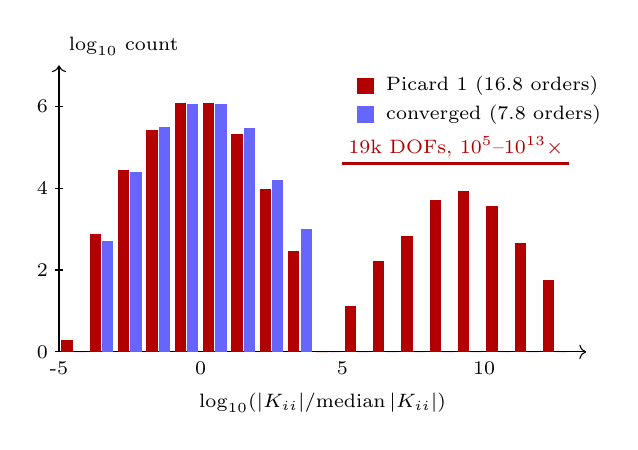
\begin{tikzpicture}[x=0.36cm,y=0.52cm]
        % axes
        \draw[->] (0,0) -- (18.6,0);
        \node at (9.3,-1.25) {\scriptsize $\log_{10}(|K_{ii}|/\mathrm{median}\,|K_{ii}|)$};
        \draw[->] (0,0) -- (0,7.0) node[above right]{\scriptsize $\log_{10}$ count};
        \foreach \y in {0,2,4,6} \draw (-0.15,\y) -- (0.15,\y) node[left=2pt]{\scriptsize \y};
        \foreach \i/\l in {0/-5,5/0,10/5,15/10} \node[below] at (\i,0) {\scriptsize \l};
        % Picard 1 (from vel_obs)
        \foreach \h [count=\i from 0] in {0.301,2.886,4.439,5.426,6.072,6.090,5.330,3.990,2.453,0,1.114,2.220,2.833,3.720,3.941,3.571,2.666,1.763}
          \fill[red!70!black] (\i+0.08,0) rectangle (\i+0.48,\h);
        % converged (last Picard iteration)
        \foreach \h [count=\i from 0] in {0,2.698,4.385,5.481,6.060,6.064,5.474,4.200,2.992,0,0,0,0,0,0,0,0,0}
          \fill[blue!60] (\i+0.52,0) rectangle (\i+0.92,\h);
        % legend
        \fill[red!70!black] (10.5,6.3) rectangle (11.1,6.7);
        \node[anchor=west] at (11.2,6.5) {\scriptsize Picard 1 (16.8 orders)};
        \fill[blue!60] (10.5,5.6) rectangle (11.1,6.0);
        \node[anchor=west] at (11.2,5.8) {\scriptsize converged (7.8 orders)};
        \draw[thick,red!70!black] (10,4.6) -- (18,4.6);
        \node[red!70!black] at (14,5.0) {\scriptsize 19k DOFs, $10^{5}$--$10^{13}\times$};
      \end{tikzpicture}
    \end{column}
    \begin{column}{0.38\textwidth}
      \begin{itemize}
        \item PETSc dumps $K$, $f$ and the MUMPS solution; a small driver
              tries solvers in seconds.
        \item First Picard matrix: diagonal spans \bad{16.8 orders of magnitude},
              with a separate cluster up to $10^{13}\times$ the median.
        \item Beyond double precision: even MUMPS only reaches $10^{-6}$ there
              (later iterations $10^{-10}$--$10^{-15}$).
      \end{itemize}
    \end{column}
  \end{columns}
\end{frame}

% =====================================================================
\begin{frame}{The cause: the initial guess, not the physics}
  \begin{columns}[c]
    \begin{column}{0.47\textwidth}
      \centering
      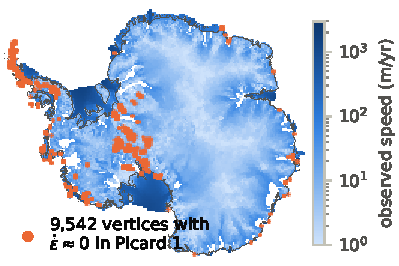
\includegraphics[width=\linewidth]{ais3_zero_strain_map.pdf}
    \end{column}
    \begin{column}{0.51\textwidth}
      \small
      \begin{itemize}
        \item The first Picard viscosity comes from \texttt{md.initialization}
              --- here the \textbf{observed velocity}, as is common.
        \item Its gap fills are \alert{piecewise constant}: 25k vertices share an
              identical $(u,v)$ with a neighbour.
        \item Constant velocity $\Rightarrow$ zero strain rate $\Rightarrow$
              $\bar\mu \propto \dot\varepsilon_e^{-2/3} \to$ huge.
        \item The orange vertices are exactly the matrix's high cluster: initial strain
              rate $\sim10^{-25}\,\mathrm{s}^{-1}$ there vs $10^{-10}$ across the ice.
      \end{itemize}
      \begin{block}{Relevant to any ISSM user}
        Initialising from observations with flat infill makes the \emph{first}
        stress-balance solve ill-conditioned --- for direct solvers too.
        \good{Smoothing it} (5 passes of neighbour averaging) removed every
        multigrid fallback.
      \end{block}
    \end{column}
  \end{columns}
\end{frame}

% =====================================================================
\begin{frame}{On the converged system, everything works}
  Last-Picard AIS3 SSA matrix (2.95M DOFs), solved outside ISSM;
  GMRES to true residual $10^{-8}$:
  \begin{center}
  \small
  \begin{tabular}{lrrr}
    \toprule
    Solver & Iterations & Time & Error vs MUMPS \\
    \midrule
    MUMPS, 16 CPU cores                       & --- & 15.7\,s & --- \\
    GAMG, 16 cores                            & 118 & 72.4\,s & $6\times10^{-6}$ \\
    GAMG + rigid-body modes, 16 cores         & 27  & 18.6\,s & $4\times10^{-7}$ \\
    \textbf{BoomerAMG, one A100 GPU}          & 110 & \good{3.1\,s} & $7\times10^{-6}$ \\
    \bottomrule
  \end{tabular}
  \end{center}
  \begin{itemize}
    \item BoomerAMG: 2.3\,s setup + 0.8\,s solve --- \good{$\sim$5$\times$} 16-core
          MUMPS, \good{$\sim$2$\times$} the 48-core MUMPS AIS3 uses ($\sim$6.3\,s).
    \item Giving GAMG the in-plane rotation mode (shelves are only pinned at
          grounding lines) cuts its iterations 4$\times$.
    \item Transient steps start from the previous velocity, so they look like this
          matrix --- confirmed over a 1-year run: no fallbacks after step 1.
  \end{itemize}
  {\scriptsize One A100 GPU = $\tfrac18$ of a DGX A100 node on NCI's Gadi (8 GPUs, 128 cores);
  a GPU job gets 16 of the cores.}
\end{frame}

% =====================================================================
\begin{frame}{Making it work inside ISSM: two fixes}
  \begin{enumerate}
    \item \textbf{Recovery mode was sticky:} after one failed solve ISSM used MUMPS
          for every later Picard iteration. \good{Fix} (C++): switch back afterwards.
    \item \textbf{Recovery on GPU data returned zero:} a host solution vector next to
          GPU matrices. \good{Fix}: recovery solver also gets \texttt{vec\_type=cuda}.
  \end{enumerate}
  \begin{columns}[c]
    \begin{column}{0.46\textwidth}
      \begin{block}{Result: continental SSA stress balance}
        \begin{itemize}
          \item Early Picard solves fail $\to$ MUMPS $\to$ \good{back to BoomerAMG};
                all 20 iterations converge.
          \item Velocity vs 48-core MUMPS: within \good{$3\times10^{-7}$}
                (99th percentile), max 0.17\,m/yr.
        \end{itemize}
      \end{block}
    \end{column}
    \begin{column}{0.52\textwidth}
      \centering
      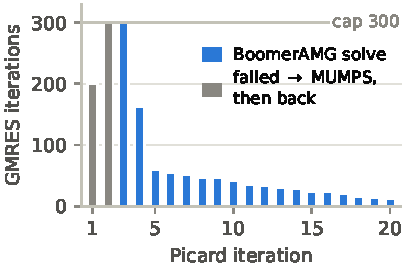
\includegraphics[width=0.95\linewidth]{picard_iterations.pdf}\\
      {\scriptsize 16 ranks + MPS, one A100 GPU}
    \end{column}
  \end{columns}
\end{frame}

% =====================================================================
\begin{frame}{The new bottleneck: everything that isn't the solve}
  \begin{columns}[T]
    \begin{column}{0.48\textwidth}
      \small
      \begin{tabular}{lrr}
        \toprule
        One stress balance & MUMPS & GPU \\
                           & 48 ranks & 1 rank \\
        \midrule
        linear solves & 125\,s & 123\,s \\
        assembly etc. & 12\,s  & \bad{600\,s} \\
        \midrule
        total         & 137\,s & 724\,s \\
        \bottomrule
      \end{tabular}
      \vspace{0.5em}

      Matrix assembly runs on CPU ranks: one rank is $\sim$50$\times$ slower.
      Need many ranks on one GPU.
    \end{column}
    \begin{column}{0.50\textwidth}
      \small
      Ranks sharing one A100 GPU (BoomerAMG, converged matrix):\\[0.2em]
      \centering
      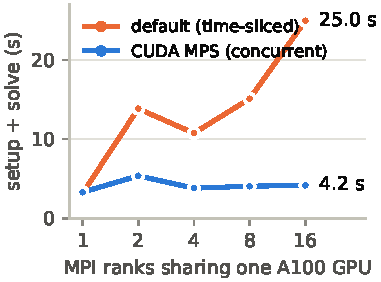
\includegraphics[width=0.95\linewidth]{mps_ranks.pdf}\\[0.2em]
      \raggedright
      Without NVIDIA's Multi-Process Service the ranks time-slice the GPU;
      with it they share it concurrently.
    \end{column}
  \end{columns}
\end{frame}

% =====================================================================
\begin{frame}{End to end: faster and cheaper than 48-core MUMPS}
  \begin{center}
  \small
  \begin{tabular}{lrr}
    \toprule
    Continental SSA, MUMPS (48 cores) $\to$ BoomerAMG (1 A100 GPU) & core time & SU \\
    \midrule
    one stress balance, observed start & 137 $\to$ 109\,s (1.3$\times$) & 4.2 $\to$ 2.8 \\
    one stress balance, smoothed start & 141 $\to$ \good{86\,s} (1.6$\times$) & 4.3 $\to$ \good{2.4} \\
    one-year transient (10 steps)      & 831 $\to$ \good{565\,s} (1.5$\times$) & 23.0 $\to$ \good{12.1} \\
    \bottomrule
  \end{tabular}
  \end{center}
  \vspace{-0.3em}
  \begin{columns}[c]
    \begin{column}{0.55\textwidth}
      \centering
      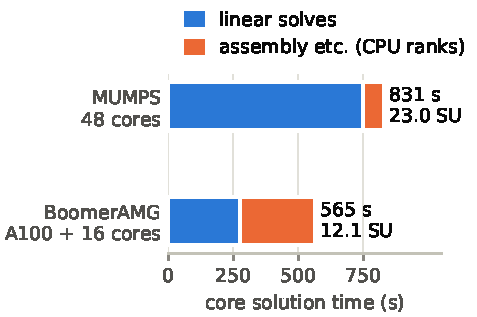
\includegraphics[width=0.85\linewidth]{breakdown_transient.pdf}
    \end{column}
    \begin{column}{0.43\textwidth}
      \small
      \begin{itemize}
        \item One-year transient (chart): same Picard iterations per step; velocity
              within $3\times10^{-7}$ (99th pct.), thickness within 1.3\,cm.
        \item One A100 GPU + 16 cores ($\tfrac18$ DGX node) $\approx$ 72\,SU/h vs
              96\,SU/h for 48 CPU cores.
        \item Assembly is now half of the GPU run's time.
      \end{itemize}
    \end{column}
  \end{columns}
\end{frame}

% =====================================================================
\begin{frame}{Take-home for ice-sheet modellers}
  \begin{enumerate}
    \item \textbf{Benchmark against what you run.} 7.6$\times$ vs 1-core MUMPS on a
          square shelf became 1.5$\times$ faster and 1.9$\times$ cheaper over a
          transient year vs 48-core MUMPS on Antarctica.
    \item \textbf{Your initial velocity shapes the linear algebra.} Flat observational
          infill gave a first matrix spanning 16.8 orders of magnitude --- it defeats
          multigrid and degrades direct solves too. Smoothing it removed every
          fallback.
    \item \textbf{Iterative solvers need a fallback that comes back.} One hard solve
          shouldn't pin a whole run to the slow path.
    \item \textbf{A faster solve exposes the rest.} On a GPU the bottleneck moved to
          assembly; CUDA MPS lets 16 CPU ranks share one GPU, which is what turned
          724\,s into 109\,s.
  \end{enumerate}
\end{frame}

% =====================================================================
\begin{frame}{Next}
  \begin{columns}[T]
    \begin{column}{0.5\textwidth}
      \textbf{SSA}
      \begin{itemize}
        \item Multi-decade projection chunks on the GPU, with the smoothed start.
        \item Assembly is now half the GPU run's time: more ranks per GPU, or
              assembly on the GPU.
      \end{itemize}
    \end{column}
    \begin{column}{0.5\textwidth}
      \textbf{Higher-order: the bigger prize}
      \begin{itemize}
        \item 23.8M vertices; MUMPS needs 1.4--2.8\,TB and hangs in long
              inversions.
        \item Same matrix-dump workflow: does BoomerAMG handle 15 thin layers,
              and does it fit in 80\,GB?
      \end{itemize}
    \end{column}
  \end{columns}
  \vspace{1.2em}
  \begin{center}
    \Large Thanks --- questions?\\[0.4em]
    {\small ISSM GPU fork: \texttt{ACCESS-NRI/ISSM}, branch \texttt{justinh2002/GPU\_cuda}
    (\texttt{test/GPU\_CHANGES.md})}
  \end{center}
\end{frame}

% =====================================================================
\appendix
\begin{frame}{Backup: why the gap grows with resolution (SquareShelf)}
  \begin{columns}[c]
    \begin{column}{0.48\textwidth}
      \begin{center}\small
      \begin{tabular}{lc}
        \toprule
        Solver & $\alpha$ in $t\propto N^{\alpha}$ \\
        \midrule
        MUMPS     & 1.39 \\
        GPU GAMG  & 1.05 \\
        hypre BoomerAMG (GPU) & 1.03 \\
        \bottomrule
      \end{tabular}
      \end{center}
    \end{column}
    \begin{column}{0.50\textwidth}
      \begin{itemize}
        \item Fit to 2\,km, 1\,km, 500\,m (one A100 GPU, one rank, one-core MUMPS).
        \item The advantage grows as $\sim N^{0.36}$: the payoff of $O(N)$ multigrid
              over factorisation.
        \item Absolute speedups depend on the baseline --- see main slides.
      \end{itemize}
    \end{column}
  \end{columns}
\end{frame}

\begin{frame}{Backup: block size and the near-null space}
  \begin{itemize}
    \item AMG must represent the matrix's low-energy modes on its coarse grids.
    \item SSA is a vector problem: the modes are \textbf{rigid-body motions} ---
          two translations and an in-plane rotation.
    \item \texttt{mat\_block\_size=2} groups each node's $(u,v)$: without it BoomerAMG
          diverges and GAMG stalls at scale.
    \item ISSM never passes node coordinates, so GAMG only knows the translations.
          Supplying the rotation (recovered by matching the dumped solution to the
          mesh) cut GAMG from 118 to 27 iterations on the AIS3 matrix.
  \end{itemize}
\end{frame}

\begin{frame}{Backup: multi-GPU and the AMG setup on GPU}
  \begin{itemize}
    \item 1\,km SquareShelf on 4 A100 GPUs: GPU GMRES 182\,s vs CPU GMRES 177\,s ---
          every GMRES iteration needs a global reduction; communication-limited.
    \item GAMG's coarse-grid products (PtAP) on the GPU hit a CUSPARSE resource
          limit with smoothed aggregation; on the host they take 200--370\,s for the
          AIS3 matrix. BoomerAMG builds its hierarchy on the GPU in 2.3\,s.
    \item This hypre build is GPU-only (no CPU BoomerAMG); native
          \texttt{mat\_type=hypre} has an open hypre 2.31 bug, so the production
          path is \texttt{aijcusparse}.
  \end{itemize}
\end{frame}

\begin{frame}{Backup: how it is switched on}
  \small
  \begin{itemize}
    \item Per-analysis PETSc options from Python, stress balance only:\\
          \texttt{vec\_type cuda, mat\_type aijcusparse, mat\_block\_size 2,}\\
          \texttt{ksp\_type gmres, ksp\_pc\_side right, ksp\_rtol 1e-8,}\\
          \texttt{pc\_type hypre, pc\_hypre\_type boomeramg, strong\_threshold 0.25}
    \item Recovery solver: MUMPS + \texttt{vec\_type cuda}. Helper:
          \texttt{gpuhypreoptions} (Python and MATLAB, \texttt{src/m/solvers}).
    \item Other analyses (mass transport, level sets) keep their defaults --- block
          size 2 would break their scalar systems.
    \item pyissm cluster subclass for the GPU queue: requests the GPU, runs $n$ MPI
          ranks on 16 cores, starts the MPS daemon.
    \item \texttt{PETSC\_OPTIONS=-use\_gpu\_aware\_mpi 0}: with ranks sharing a GPU,
          MPI's GPU-direct copies crashed a transient; staging through the host
          cost nothing measurable.
  \end{itemize}
\end{frame}

\end{document}
